\documentclass{article}

%=======================Title settings=======================
\title{SWT - Mandatory Assigment 2 : ATM}
\author{Gruppe 16}
\date{\today}

%=======================Use Package==========================
\usepackage[utf8]{inputenc}
\usepackage{natbib}
\usepackage{graphicx}
\usepackage{float}
\usepackage{amsmath}
\usepackage{amsfonts}
\usepackage{amssymb}
\usepackage{graphicx}
\usepackage{booktabs}
\usepackage{listings}
\usepackage{xcolor}
\usepackage{hyperref}
\usepackage{comment}
\usepackage{hyperref}
%=======================Package settings=======================

\hypersetup{
    colorlinks,
    citecolor=black,
    filecolor=black,
    linkcolor=black,
    urlcolor=blue
}

\lstset{
  language=Matlab,                % choose the language of the code
  numbers=left,                   % where to put the line-numbers
  stepnumber=1,                   % the step between two line-numbers.        
  numbersep=5pt,                  % how far the line-numbers are from the code
  backgroundcolor=\color{white},  % choose the background color. You must add \usepackage{color}
  showspaces=false,               % show spaces adding particular underscores
  showstringspaces=false,         % underline spaces within strings
  showtabs=false,                 % show tabs within strings adding particular underscores
  tabsize=2,                      % sets default tabsize to 2 spaces
  captionpos=b,                   % sets the caption-position to bottom
  %caption={Kode udsnit fra main.c programmet til opgave 1},
  %label=mainOpg1
  breaklines=true,                % sets automatic line breaking
  breakatwhitespace=true,         % sets if automatic breaks should only happen at whitespace
  belowcaptionskip=1\baselineskip,
  %frame=L,
  xleftmargin=\parindent,
  basicstyle=\footnotesize\ttfamily,
  keywordstyle=\bfseries\color{blue},
  commentstyle=\itshape\color{teal},
  identifierstyle=\color{black},
  stringstyle=\color{red},
}


%=======================Page settings=======================
\topmargin 0.0cm
\oddsidemargin 0.2cm
\textwidth 16cm 
\textheight 21cm
\footskip 1.0cm


\begin{document}
%=======================Title========================
\maketitle

\begin{table}[H]
\centering
\begin{tabular}{|l|l|l|}
\hline
\textbf{Navn}       & \textbf{Studieretning} & \textbf{Student Number} \\ \hline
Sivert Sømmer Sagmo & IKT                    & 201608544             \\ \hline
Glenn Laursen & IKT                    & 201703930             \\ \hline
Saeed Soltani & IKT                    & 201710716             \\ \hline
\end{tabular}
\end{table}

\tableofcontents
\pagebreak
%=======================Sections=======================

\section{Genaflevering}
vi har fuldført vores program hvor vi har opdateret funktioner, der opdater flyets velocity og compasscourse. dernæst har vi lavet test til udvidelsen af programmet. De test vi har lavet er blevet udvidet. Flere test er blevet lagt til og boundary value analysis er blevet lavet. vi har opdateret vores design med et nyt klasse diagram og et nyt sekvens diagram der afspeljer vores kode. der er tilføjet et kapitel mere i vores journal "Test"
\section{Indledning}
i denne journal har vi oprettet et ATM(Air traffic monitoring) system. hvor vi får fly med position og hastighed som en liste og valider om den tilhører et given airspace og hvor de er placeret i forhold til hinanden. dernæst har vi lavet test til de forskellige opgaver i vores system. disse test er blevet unit testet gennem jenkins.


\section{Design}
\begin{figure}[H]
	\centering
	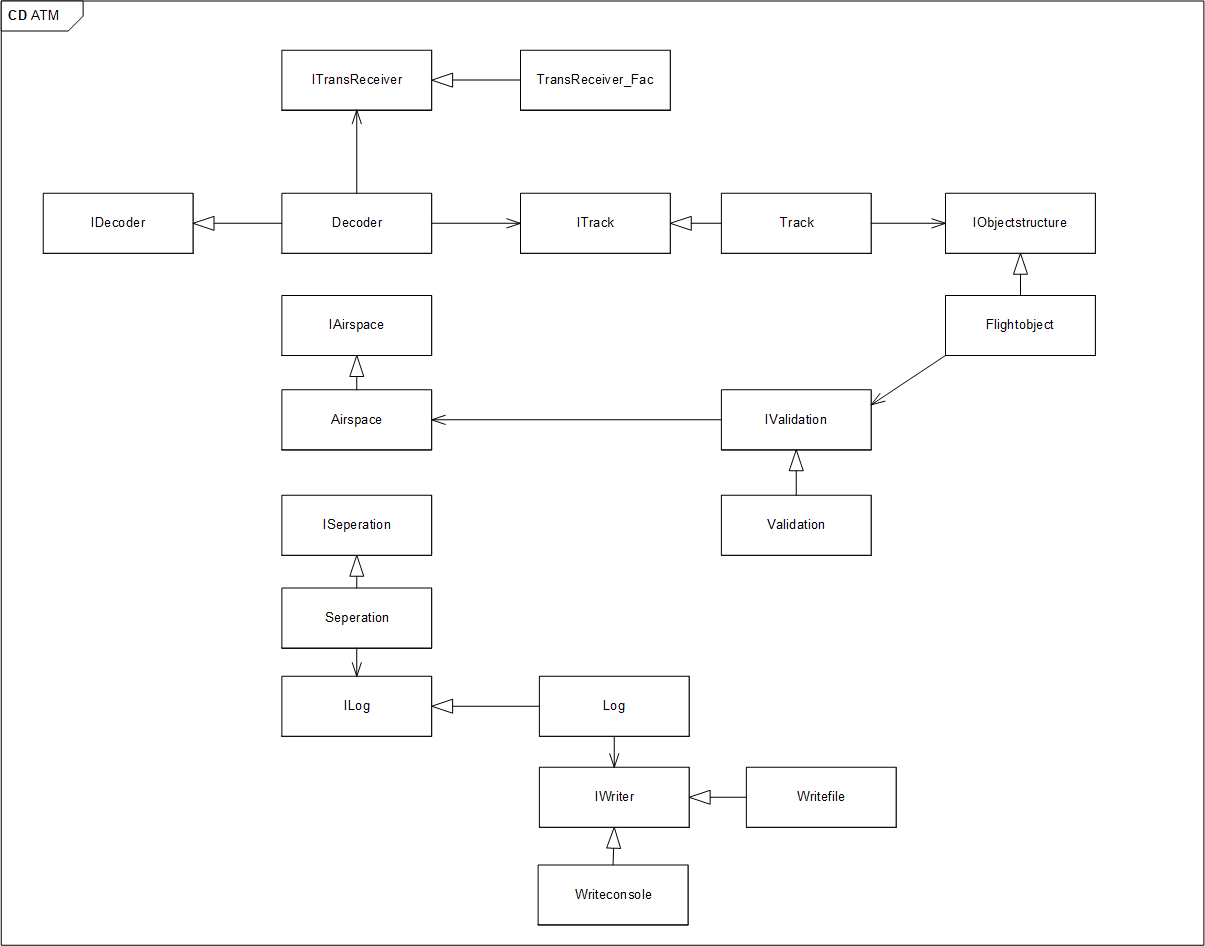
\includegraphics[width=1\linewidth]{../Diagrammer/CD_ATM}
	\caption{Klasse diagram over ATM}
	\label{fig:cdatm}
\end{figure}

\subsection{Decoder}
Decoder opgave er at tage imod beskeder fra Transreceiver. Derefter dele beskederne op i tag, X-koordinat, Y-koordinat, Altitude og Time. Dette data bruges til at oprette Tracks der indsættes i en objektstruktur
\subsection{Track}
Track opgave er at opdele en streng også oprette et nyt track som den tilfører et tag variable, X-koordinat variable, Y-koordinat variable, Altitude variable, Timestamp variable, Velocity variable og Compass course variable med henholdsvis den korrekte type. denne her variable kan så opdateres ved brug af set metoden og dens specifikke variable kan tilgås ved hjælp af get.
\subsection{IObjectstructure}
vores tracks bliver så lagt til en objektstruktur før den her objektstruktur lægger ind den given track, tager den og tjækker ved hjælp af validate funktionen om den given track er inden for vores airspace. hvis den er i det given airspace tjekker den så om det givene track allerede er i objektstrukturen. hvis den er det så opdatere den det given track for ikke at lave duplicate. hvis den ikke er til stede i objektstrukturen så lægger den det given track ind i objektstrukturen
\subsection{Validation}
Validation tager et Airspace der har et defineret område. dernæst har den en validate funktion der tager en ITrack ind som parameter. dernæst bliver track elementets altitude sammenlignet med vores boundary værdier (lower boundary og upper boundary) samt at dens x-koordinat og y-koordinat er inden for airspacets bestemte x og y parameter. de her 3 tester er af typen bool validate returner så de her 3 resultater sammen med en AND operator som giver os true i det tilfælde at alle 3 testne er true og giver os false hvis kun en af dem er false. på den måde ved vi at hvis validate retunere true vil vores track som validate tager ind som parameter være inden for vores airspace
\subsection{Airspace}
Airspace definere vores boundary værdier for de områder hvor vi er interesseret i logføre alle fly. måden det gøres på er at den tager en x og y størrelse, der definere den 2D udstrækning af vores airspace. dernæst tager den også en lower boundary og upper boundary der definere vores 3D airspace. lower boundary er fra jorden og til starte højden af vores airspace. upper boundary er højden på vores airspace. vi kan tilgå airspacets størrelser ved hjælp af set og get funktioner.
\subsection{Transreceiver-Fac}
vi får dataen fra alle fly der sender ud et transponder og bliver modtaget af en receiver. den her data bliver så behandlet af vores decoder der afventer data gennem en event.
\subsection{Seperation}
seperation tager ind en liste over alle fly der er i airspacet og tjekker x og y koordinater mod hinanden. hvis den horisontale distance og vertikal distance er inden for et given område. så sender den ud en seperation warning event.
\subsection{Log}
log subscriber til seperation og decoder. når der bliver sendt et event fra seperation skriver den så den data ind i en fil og dernæst til konsollen. når den modtager et event fra decoder skriver den, den data ud til konsollen 


\begin{figure}[H]
	\centering
	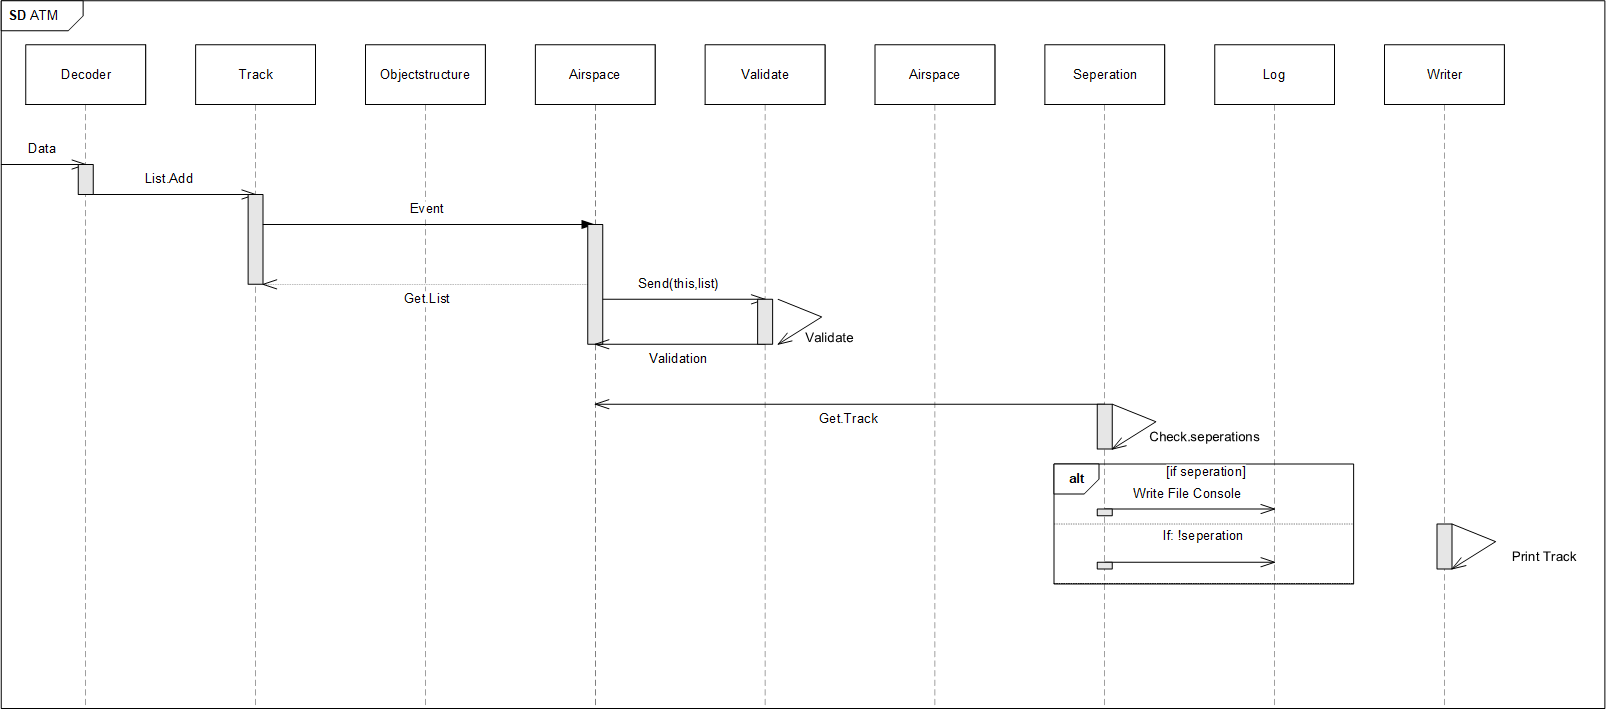
\includegraphics[width=1\linewidth]{../Diagrammer/SD_ATM}
	\caption{Sekvens diagram over ATM}
	\label{fig:sdatm}
\end{figure}

\section{Fordeling}
Da vi skulle designe vores ATM så sad vi sammen hvordan vores ATM system skulle designes. Der var ikke så mange uenigheder så det punkt kom vi forbi hurtigt. da vi skulle til at implementere klasser så var der ofte et problem med at mødes og få tid til det. Gruppe medlemmerne havde ofte nogle vigtige aftaler som at flytte ind eller job samtale eller sygdom. Derfor har vi ikke rigtig aftalt om hvorfor vi lige præcis har fordelt implementering og test som vi har gjort. Derimod de dage hvor vi har haft tid sat os sammen og hjulpet hinanden selvom det ikke var vores job at implementere og teste en anden persons arbejde. det ikke den mest optimale måde, men det var den bedste løsning vi kunne komme med pga tidsmangel. 
\section{CI Server}
Inden da vi skulle Unit teste vores kode fik vi sat vore jenkins server op. Det var ikke et problem da der var en guide på blackboard på hvordan vi satte coverage templaten op. Problemet opstod først da jenkins ikke understøttede .NETCORE 3.0 frameworket. Vi prøvede på at nedgrader til .NETCORE 2.2 det hjalp lidt på vores problem. Derefter manglede vi mange packages unødvendige packages. Da vi fik installeret alle packages løb vi ind i et andet problem. Nu opstod der et fejl med NUnit.Engine. Vi prøvede på at google løsninger til dette problem men vi fandt aldrig et svar til det. Så vi besluttede os for at ændre til .NET framework da jenkins serveren var sat op til .NET frameworket. Nu opstod der et nyt mystisk problem. vi prøvede på at bygge på jenkins, resultatet sagde at alt var rigtigt men kasserne var markeret svagt rødt. Vi kiggede efter feedback fra jenkins men den sagde alt var rigtigt. vi fandt så frem til at vi skulle flytte alle vores visual studio filer til roden af vores repository. dette fixede problemet og nu var jenkins serveren sat op.\\
\medskip
En ting Jenkins serveren har hjulpet os med er at den viser hvor mange procent af vores projekt vi har testet hvis vi f.eks. tager udgangspunkt i klassen Track så viste den på et tidspunkt at vi har testet 50\% af klassen Track. Man kunne også dykke længere ned i klassen for at se hvilke specefik funktioner der mangler at testes. 



\section{Konklusion}
Vi har oprettet et ATM system der indtager en liste med fly. vi har så lavet et overvågnings system for de fly der er inden for de given airspace. og lavet en overvågning over de en potentiel seperation situation mellem objektene i vores airspace. dernæst har vi testet funktionerne der har vha unit test og testne er kørt på jenkins. vi har lavet test for samtlige relevante klasser med undtagelse af writer. det har givet os et godt overblik over udviklings forløbet til vores system.

%=======================Ex. Inserts====================

%\begin{figure}[h!]
%\centering
%\includegraphics[scale=1.7]{universe}
%\caption{The Universe}
%\label{fig:universe}
%\end{figure}

%\begin{lstlisting}[caption=Caption here]
%\end[lstlisting]

% \begin{equation}
%     H(s) = \frac{s + \omega_1}{s + \omega_2}
%     \label{eq:3.14}
% \end{equation}



%\bibliographystyle{plain}
%\bibliography{references}
\end{document}